\documentclass{article}
\usepackage[utf8x]{inputenc}
\usepackage{tikz}
  \usetikzlibrary{calc}

\begin{document}

\section{Linia mijlocie într-un triunghi}

\begin{tikzpicture}
  % vîrfurile triunghiului
  \coordinate[label=left:A] (A) at (0,0);
  \coordinate[label=right:B] (B) at (5,-1);
  \coordinate[label=C] (C) at (4,2.7);

  % triunghiul
  \draw (A) -- (B) -- (C) -- cycle;
  % linia mijlocie
  \draw ($(A)!0.5!(C)$) -- ($(B)!0.5!(C)$);
\end{tikzpicture}

\textbf{1 Exercițiu: construiți celelalte linii mijlocii.}

\newpage

\section{Mediana și înălțimea într-un triunghi}

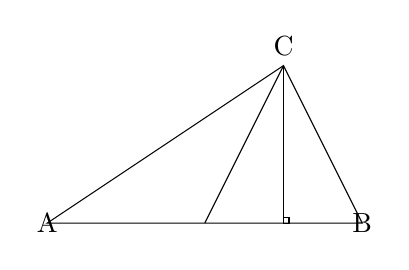
\begin{tikzpicture}
  % triunghiul
  \draw (0,0) node (A) {A}  -- (4,0) node (B) {B} -- (3,2) coordinate[label=above:C] (C) -- cycle;
  
  % mediana
  \draw ($(A)!0.5!(B)$) -- (C);
  % înălțimea
  \draw ($(A)!(C)!(B)$) coordinate (Cprim) -- (C);  
  % unghiul drept
  \draw (Cprim) rectangle ++(2pt,2pt);
\end{tikzpicture}

\textbf{2 Exercițiu:} construiți celelalte mediane și înălțimi.

\newpage

\section{Unghiuri}

\begin{tikzpicture}
  \coordinate[label=left:A] (A) at (0,0);
  \coordinate[label=right:B] (B) at (5,-1);
  \coordinate[label=C] (C) at (4,2.7);

  \draw (A) -- (B) -- (C) -- cycle;
  
  \begin{scope}
    \clip (A) -- ($(A)!1.1cm!(C)$) -- ($(A)!1.1cm!(B)$) -- cycle;
    \draw (A) circle (1);
  \end{scope}
\end{tikzpicture}

\textbf{3 Exercițiu:} Marcați celelalte unghiuri.

\end{document}